\usetikzlibrary{shapes,arrows,positioning,calc}
\begin{figure}[ht]
\centering
    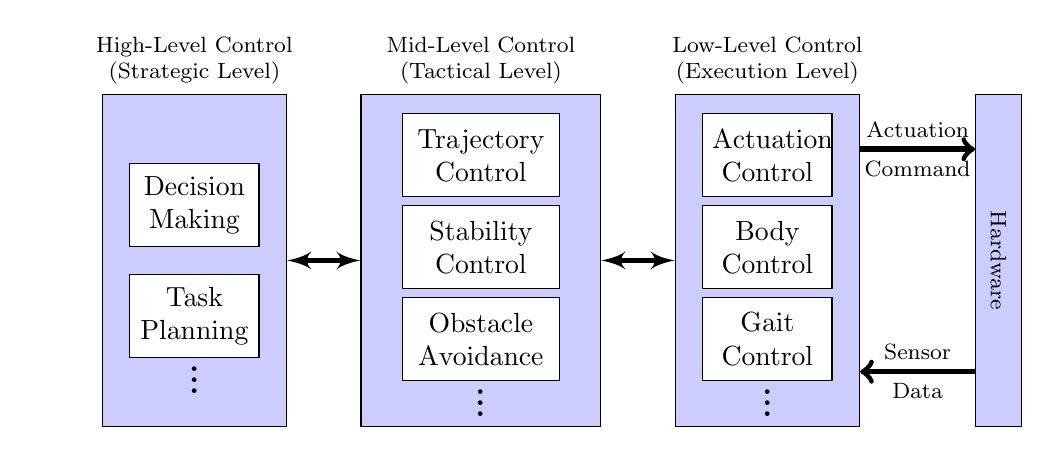
\begin{tikzpicture}[
        node distance = 3cm,
        auto,
        block/.style = {rectangle, draw, fill=blue!20, text width=8em, minimum height=12em},
        block0/.style = {rectangle, draw, fill=blue!20, text width=6em, minimum height=12em},
        block1/.style = {rectangle, draw, fill=blue!20, text width=1em, minimum height=12em},
        smallblock/.style = {rectangle, draw, fill=white, text width=5em, text centered, minimum height=3em},
        smallblock0/.style = {rectangle, draw, fill=white, text width=4em, text centered, minimum height=3em},
        line/.style = {draw, -latex'}
    ]
    
        % Place nodes
        \node [block0] at (0,0)(high) {};
        \node[align=center, font=\footnotesize, above=0em of high, text width=4cm]{High-Level Control\\ (Strategic Level)};
        \node [smallblock0] at ($(high.center) + (0, 2em)$) (highsub1) {Decision Making};
        \node [smallblock0] at ($(high.center) + (0,-2em)$) (highsub2) {Task Planning};
        \node [font=\huge] at ($(highsub2.south) + (0,-0.5em)$) {\vdots};
        
        \node [block] at ($(high.east) + (7em,0)$) (mid) {};
        \node[align=center, font=\footnotesize, above=0em of mid, text width=4cm]{Mid-Level Control \\ (Tactical Level)};
        \node [smallblock] at ($(mid.center) + (0,3.8em)$) (midsub1) {Trajectory Control};
        \node [smallblock] at ($(midsub1.south) + (0,-1.8em)$) (midsub2) {Stability Control};
        \node [smallblock] at ($(midsub2.south) + (0,-1.8em)$) (midsub3) {Obstacle Avoidance};
        \node [font=\huge] at ($(midsub3.south) + (0,-0.5em)$) {\vdots};

        \node [block0] at ($(mid.east) + (6em,0)$)(low) {};
        \node[align=center, font=\footnotesize, above=0em of low, text width=4cm]{Low-Level Control\\ (Execution Level)};
        \node [smallblock0] at ($(low.center) + (0,3.8em)$) (lowsub1) {Actuation Control};
        \node [smallblock0] at ($(lowsub1.south) + (0,-1.8em)$) (lowsub2) {Body Control};
        \node [smallblock0] at ($(lowsub2.south) + (0,-1.8em)$) (lowsub3) {Gait Control};
        \node [font=\huge] at ($(lowsub3.south) + (0,-0.5em)$) {\vdots};
        
        \node [block1] at ($(low.east) + (5em,0)$) (hardware) {};
        \node[rotate=-90, align=center, font=\footnotesize]at (hardware.center){Hardware};
        
        % % Draw edges
        \draw [line width=2pt, >=latex', <->] (high.east) -- (mid.west);
        \draw [line width=2pt, >=latex', <->] (mid.east) -- (low.west);
        \draw [line width=2pt,->] ($(low.north east) + (0,-2em)$) -- node[font=\footnotesize,above] {Actuation}node[font=\footnotesize,below] {Command}($(hardware.north west) + (0,-2em)$);
        \draw [line width=2pt,->] ($(hardware.south west) + (0,2em)$) -- node[font=\footnotesize,above] {Sensor}node[font=\footnotesize,below] {Data}($(low.south east) + (0,2em)$);
    
    \end{tikzpicture}
    \caption{Hierarchical control levels in quadruped robots.}
    \label{fig:hierarchy}
\end{figure}
